\documentclass[titlepage]{article}
\usepackage[tc]{titlepic}
\usepackage{graphicx}
\usepackage{amsmath}
\usepackage[top=25mm, bottom=25mm, left=27mm, right=27mm]{geometry}
\usepackage{caption}
\usepackage{listings}
\usepackage{lstlangarm}
\usepackage{tabu}
\usepackage[outdir=./]{epstopdf}


\date{}
\author{Ali Bahadır Bulut\\ \#041602017  \and Alp
	Gokcek \\ \#041701014 \and Erdal Sidal Dogan \\ \#041702023}
\title{
\includegraphics[width=0.6\textwidth]{../images/logo_en_color.png}\\ 
\vspace{5em}
EE306 - Microprocessors\\
\vspace{2em}
\textbf{Term Project \linebreak Sliding Text
}\\
\vspace{1.5em}
June 8, 2020}

\begin{document}
	\maketitle
	\section{Project Description}
	2-3 cümlelik abstract/description (0-1): açıklayıcı, net olmalı.
	Lorem ipsum dolor sit amet, consectetur adipiscing elit. Integer at lectus est. Etiam pellentesque, dui eget tempor suscipit, turpis dui pharetra sapien, vel molestie enim felis ac est. Aliquam erat volutpat. Duis eget dictum lacus, nec luctus magna. Sed et cursus erat. Vivamus lobortis sollicitudin fringilla. In tincidunt mi arcu, quis suscipit metus hendrerit vitae. Sed ut libero sit amet orci pretium fermentum sit amet eu augue. Vivamus lobortis ante ut nunc porta posuere. Quisque vel leo a dui ultrices imperdiet.\\
	
	Our design supports the characters provided in Figure \ref{supported_chars}.\\
	
	\begin{figure}[h]
		\centering
		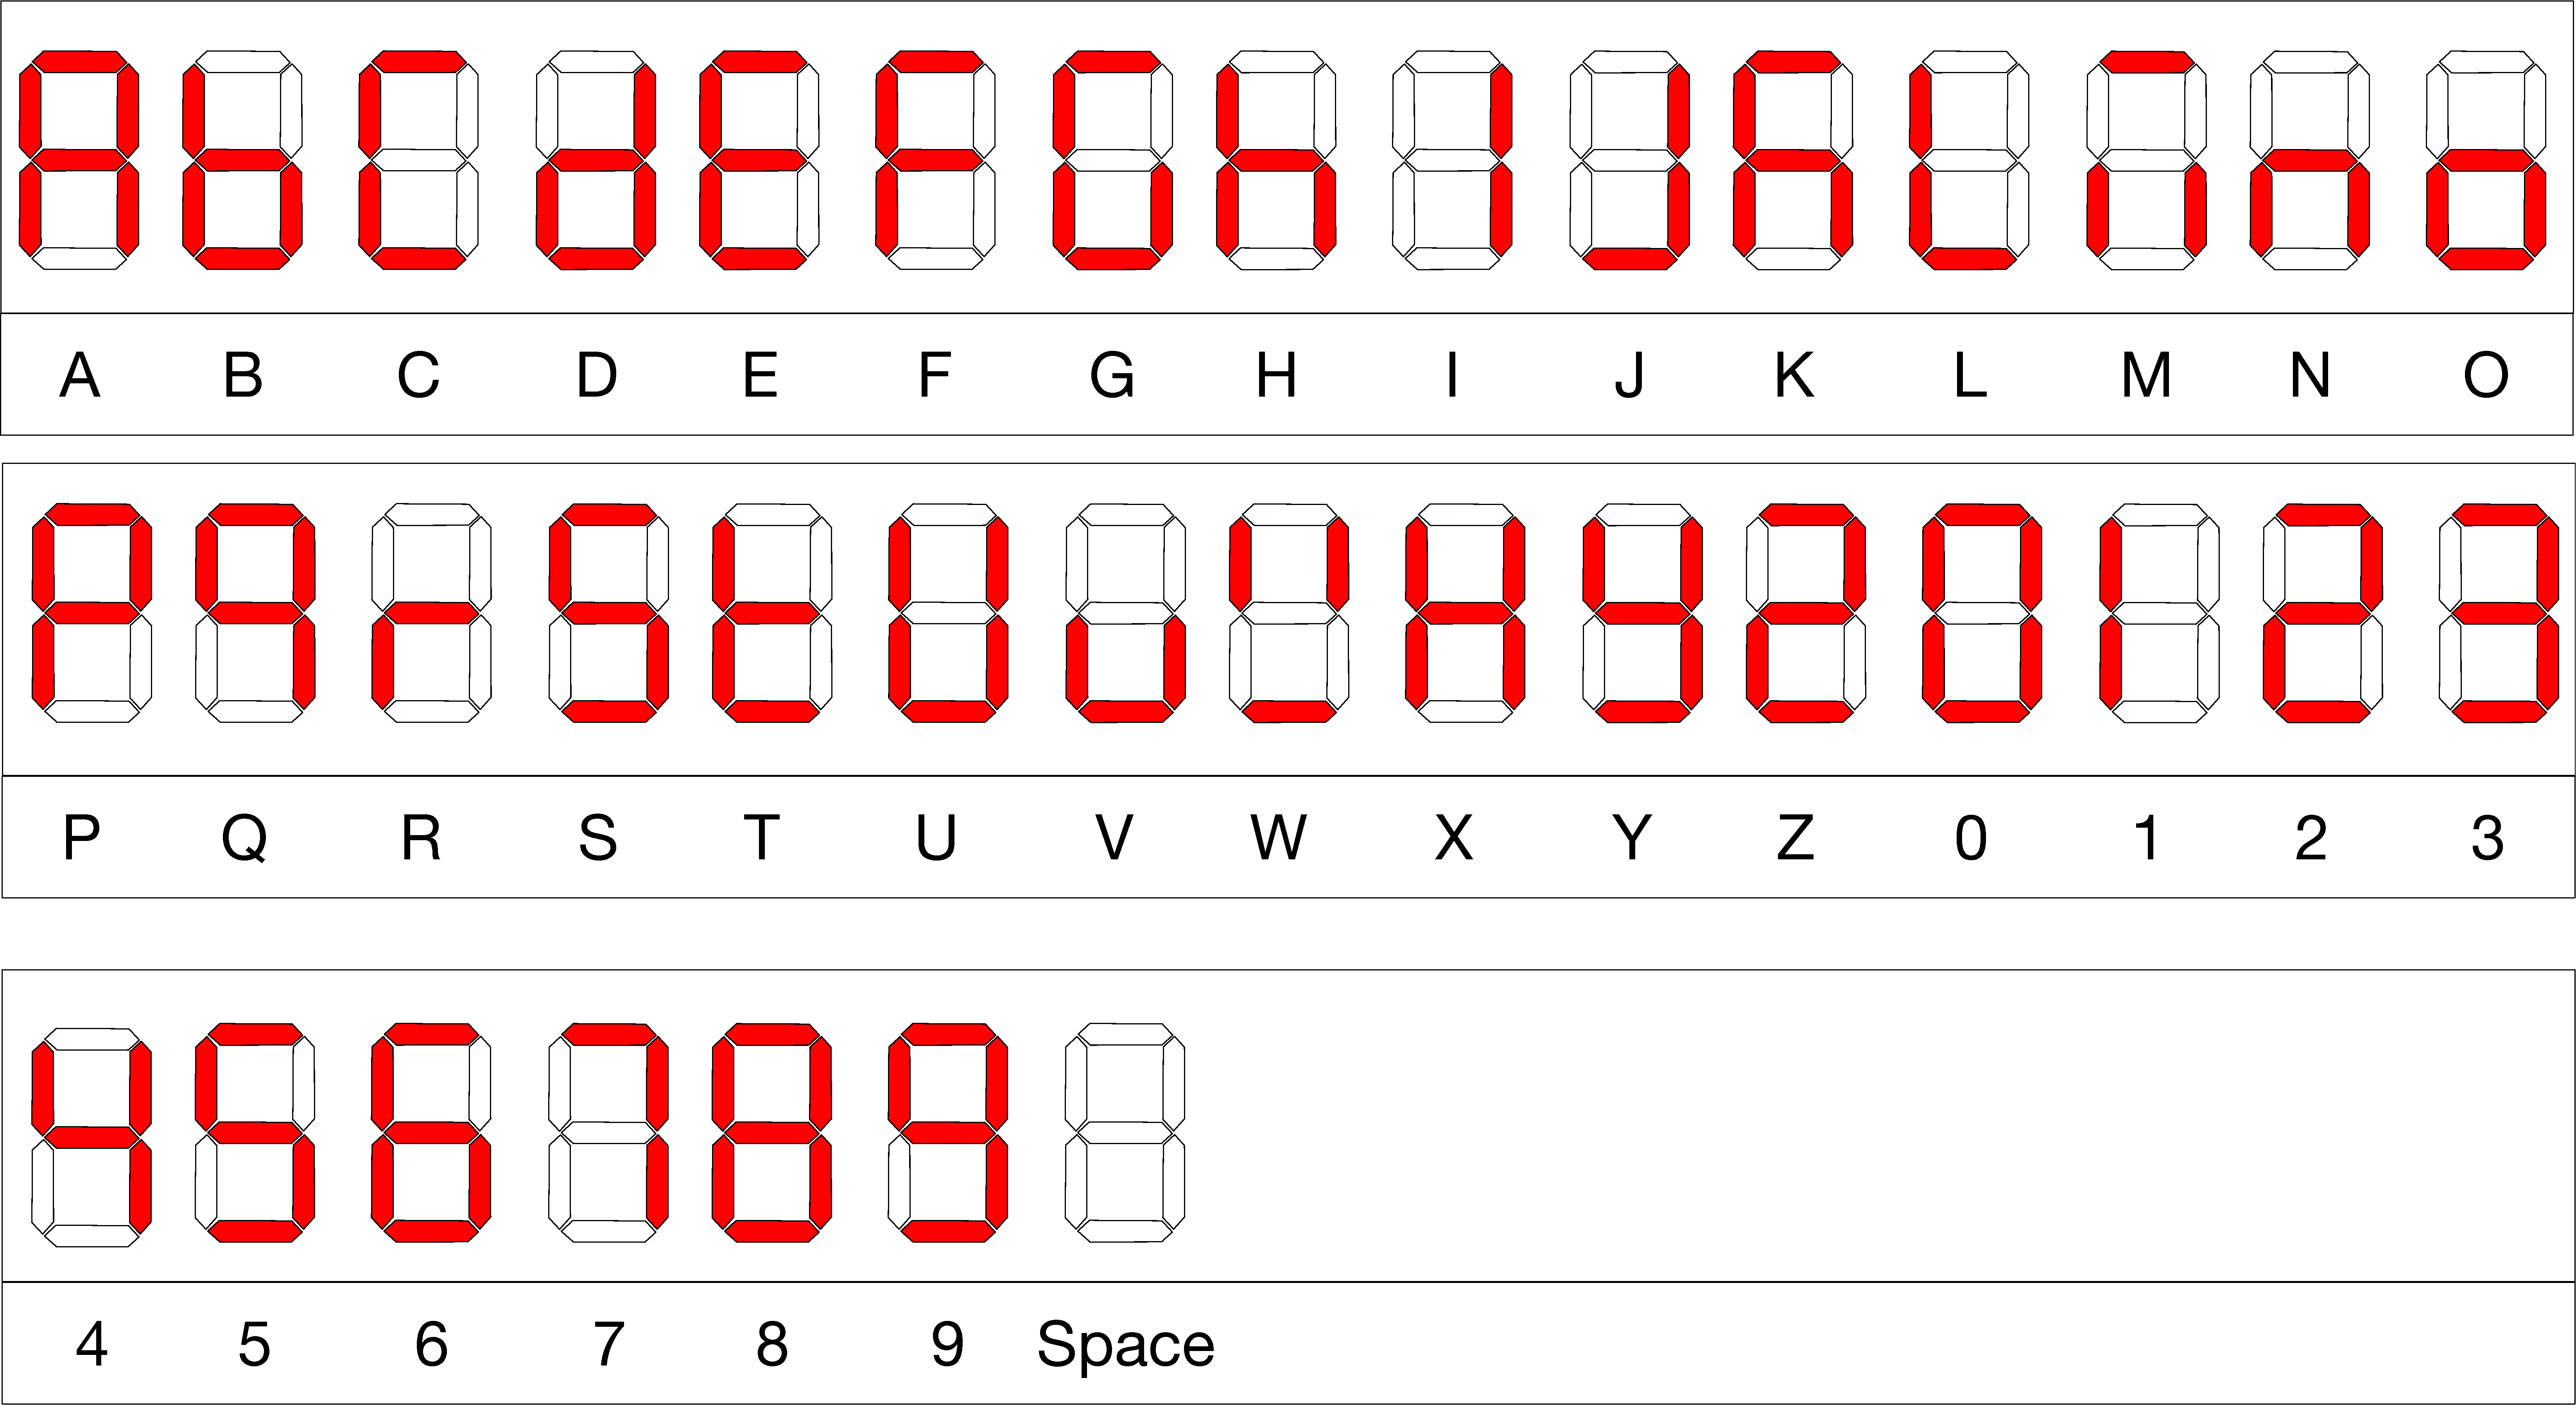
\includegraphics[scale=.1]{../images/supported_chars.pdf}
		\caption{Sample output on 7-segment displays for input "EE306 Fun"}
		\label{supported_chars}
	\end{figure}
	\section{Sample Output}
	\begin{figure}[h!]
		\centering
		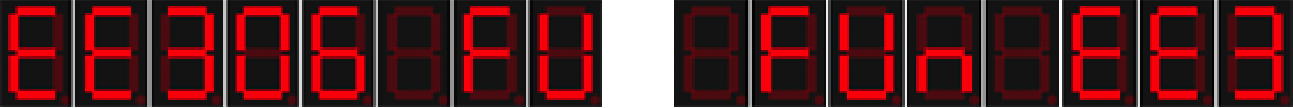
\includegraphics[scale=.45]{../images/fig1.png}
		\caption{Sample output on 7-segment displays for input "EE306 Fun"}
	\end{figure}

	\begin{figure}[h!]
		\centering
		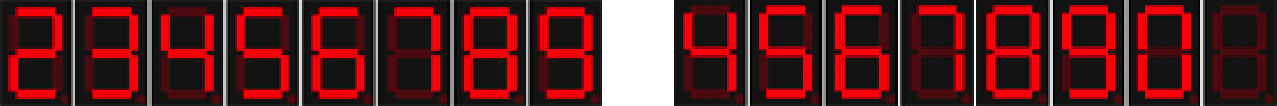
\includegraphics[scale=.45]{../images/fig2.png}
		\caption{Sample output on 7-segment displays for input "1234567890"}
	\end{figure}
	
	\begin{figure}[h!]
		\centering
		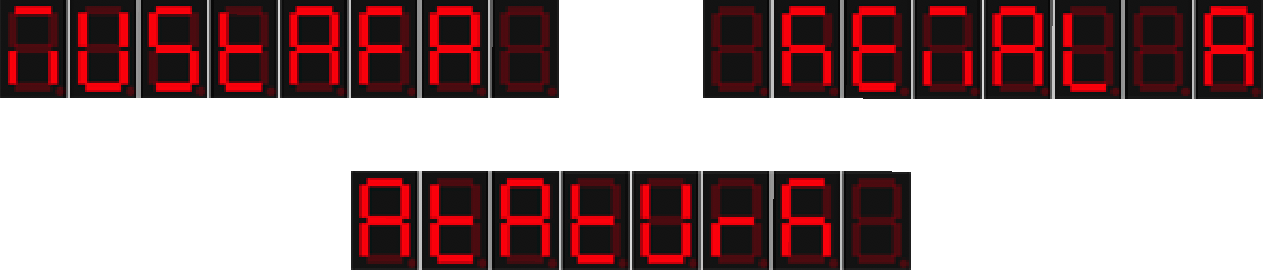
\includegraphics[scale=.45]{../images/fig3.png}
		\caption{Sample output on 7-segment displays for input "Mustafa Kemal Ataturk"}
	\end{figure}
	\section{Source Code}
	\lstinputlisting[language={[ARM]Assembler}, frame=single, basicstyle=\ttfamily, breaklines=true, showspaces=false, showstringspaces=false, caption=Source code of our sliding text project]{../source_codes/final_code.s} \label{source_code}
	
	\section{Flowcharts}
	\begin{figure}[h]
		\centering
		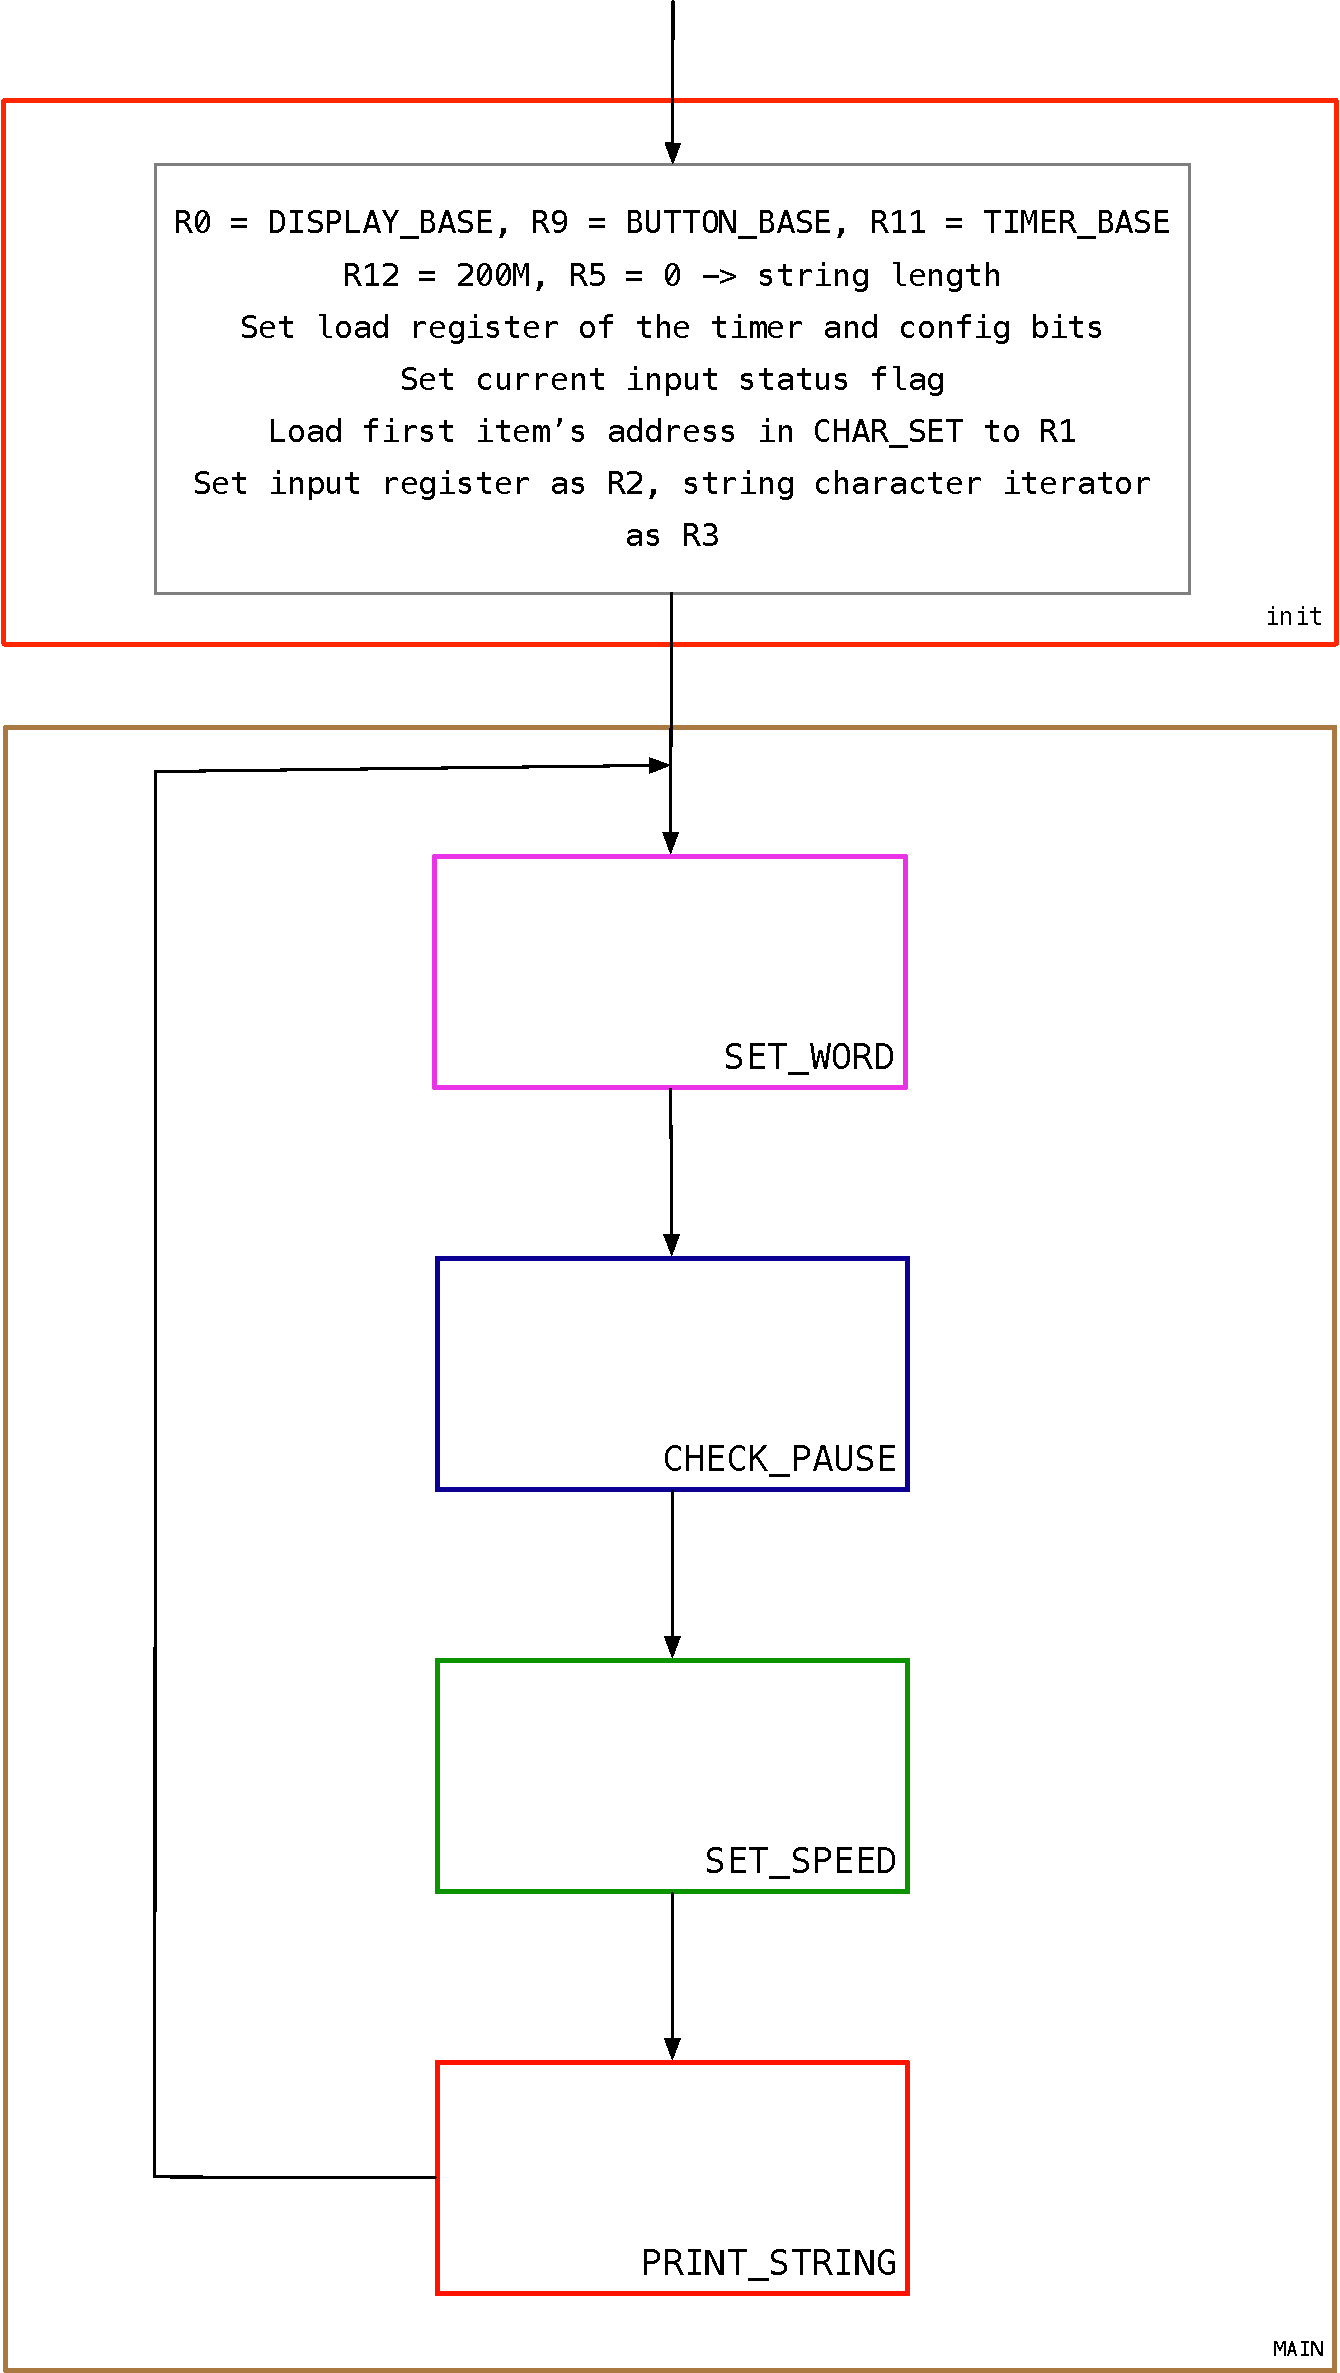
\includegraphics[scale=.27]{../images/main.pdf}
		\caption{Flowchart of Main Loop}
	\end{figure}
	\begin{figure}[h]
		\centering
		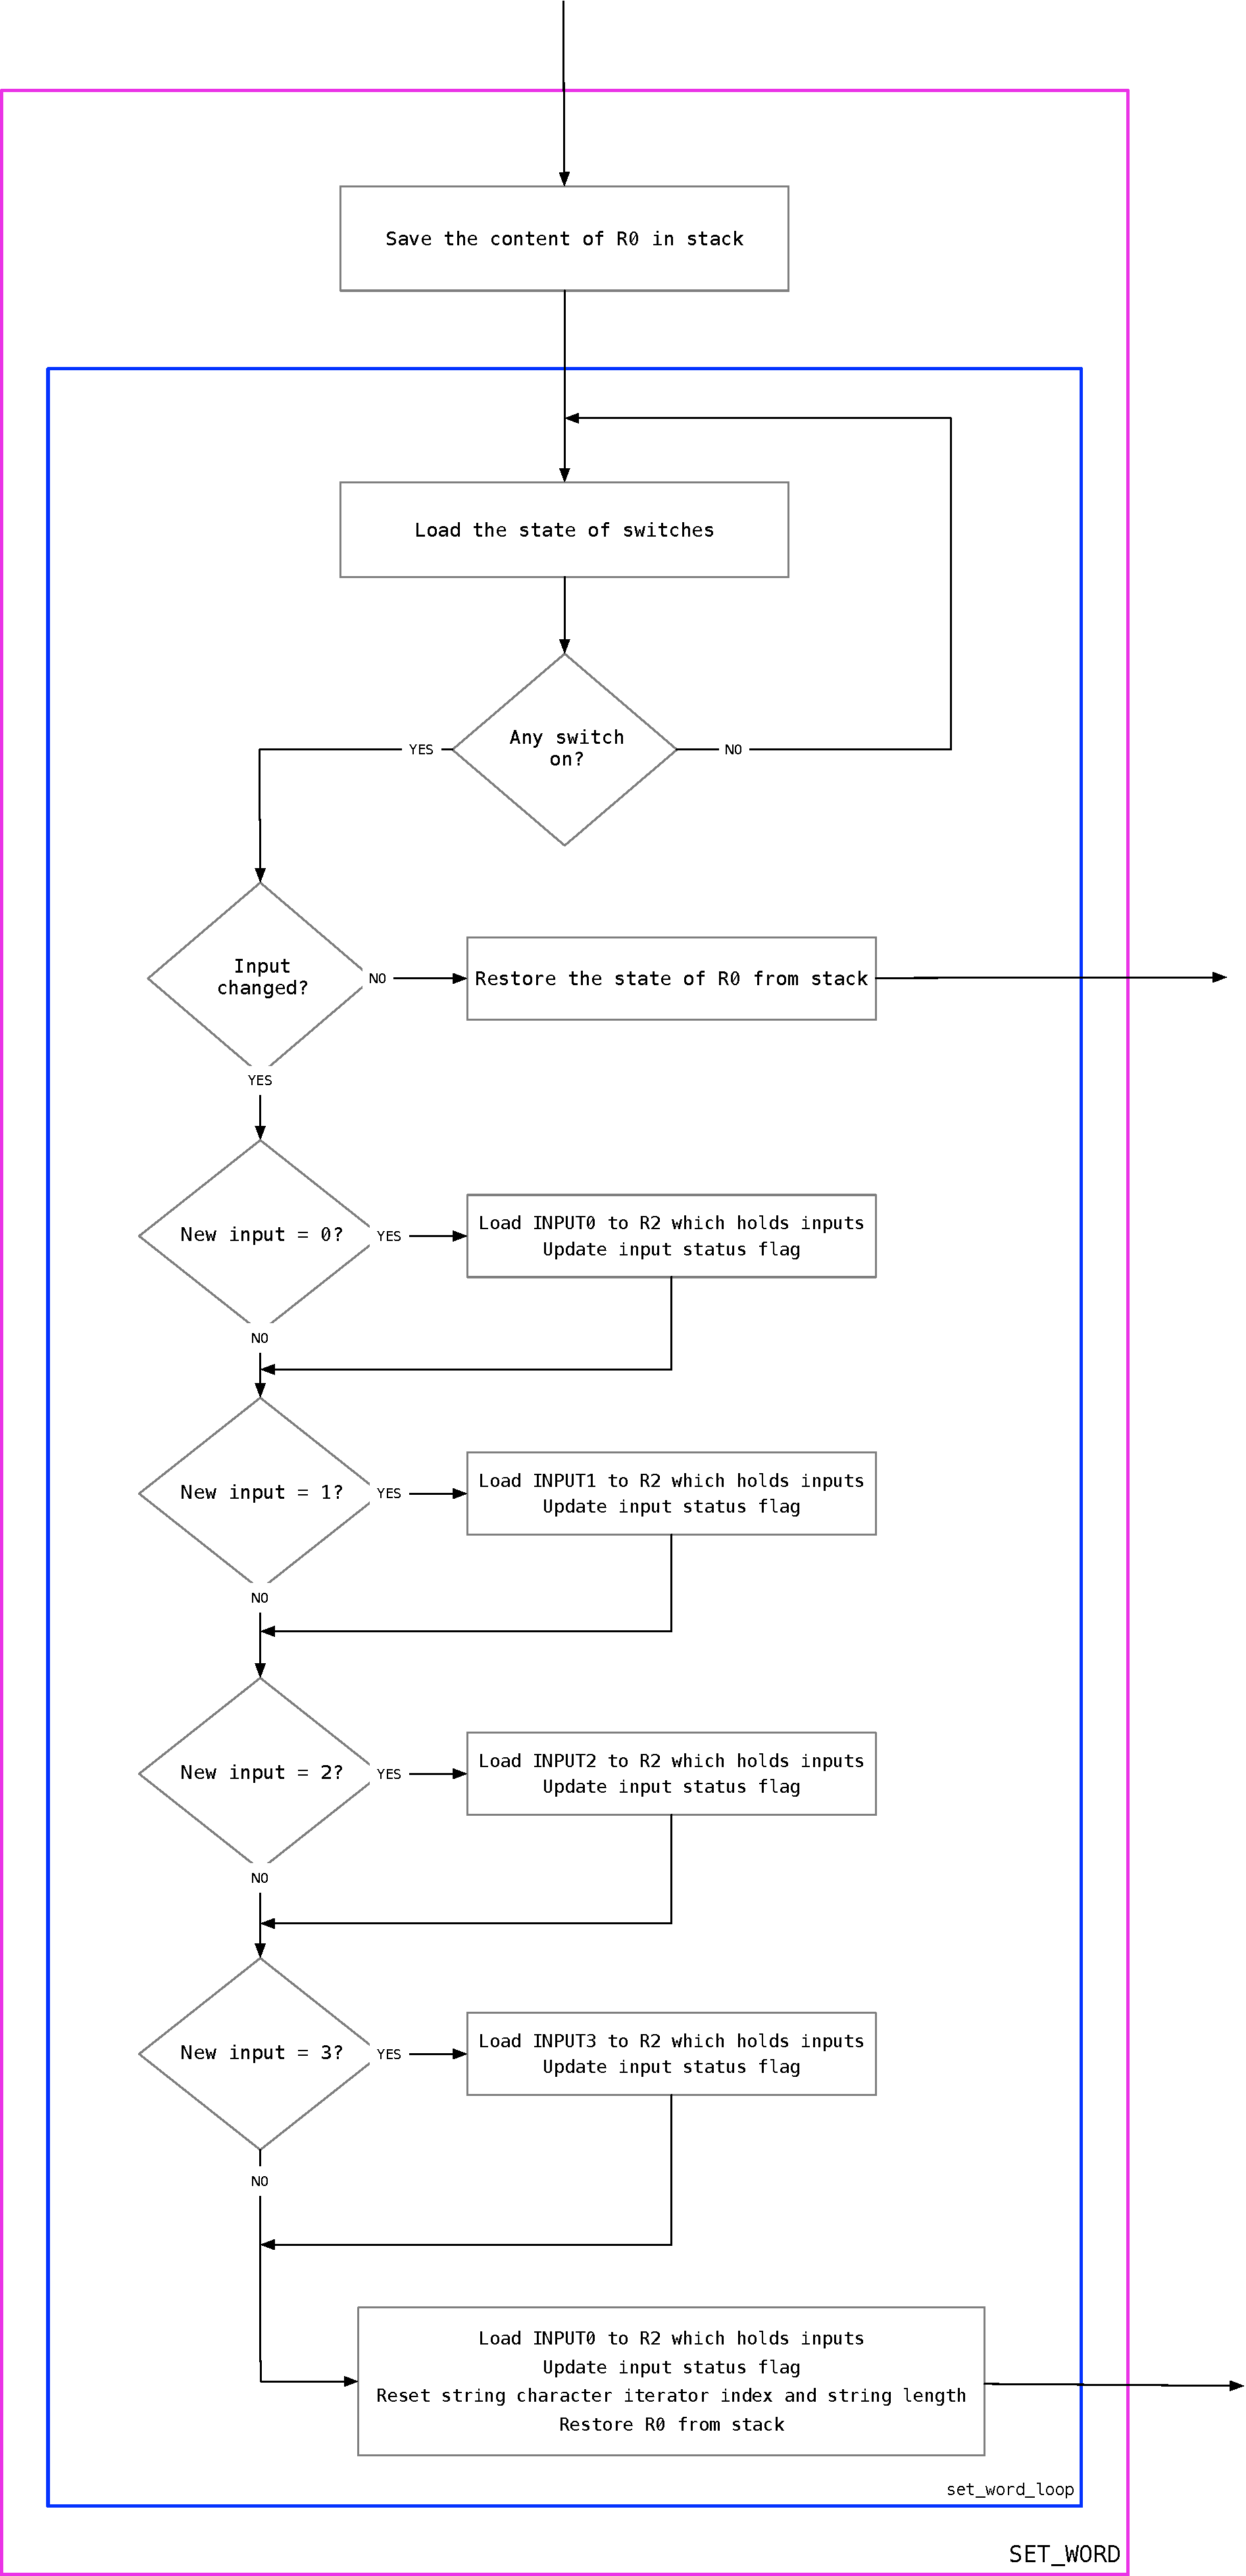
\includegraphics[scale=.3]{../images/set_word.pdf}
		\caption{Flowchart of Set Word Subroutine}
	\end{figure}
	\begin{figure}[h]
		\centering
		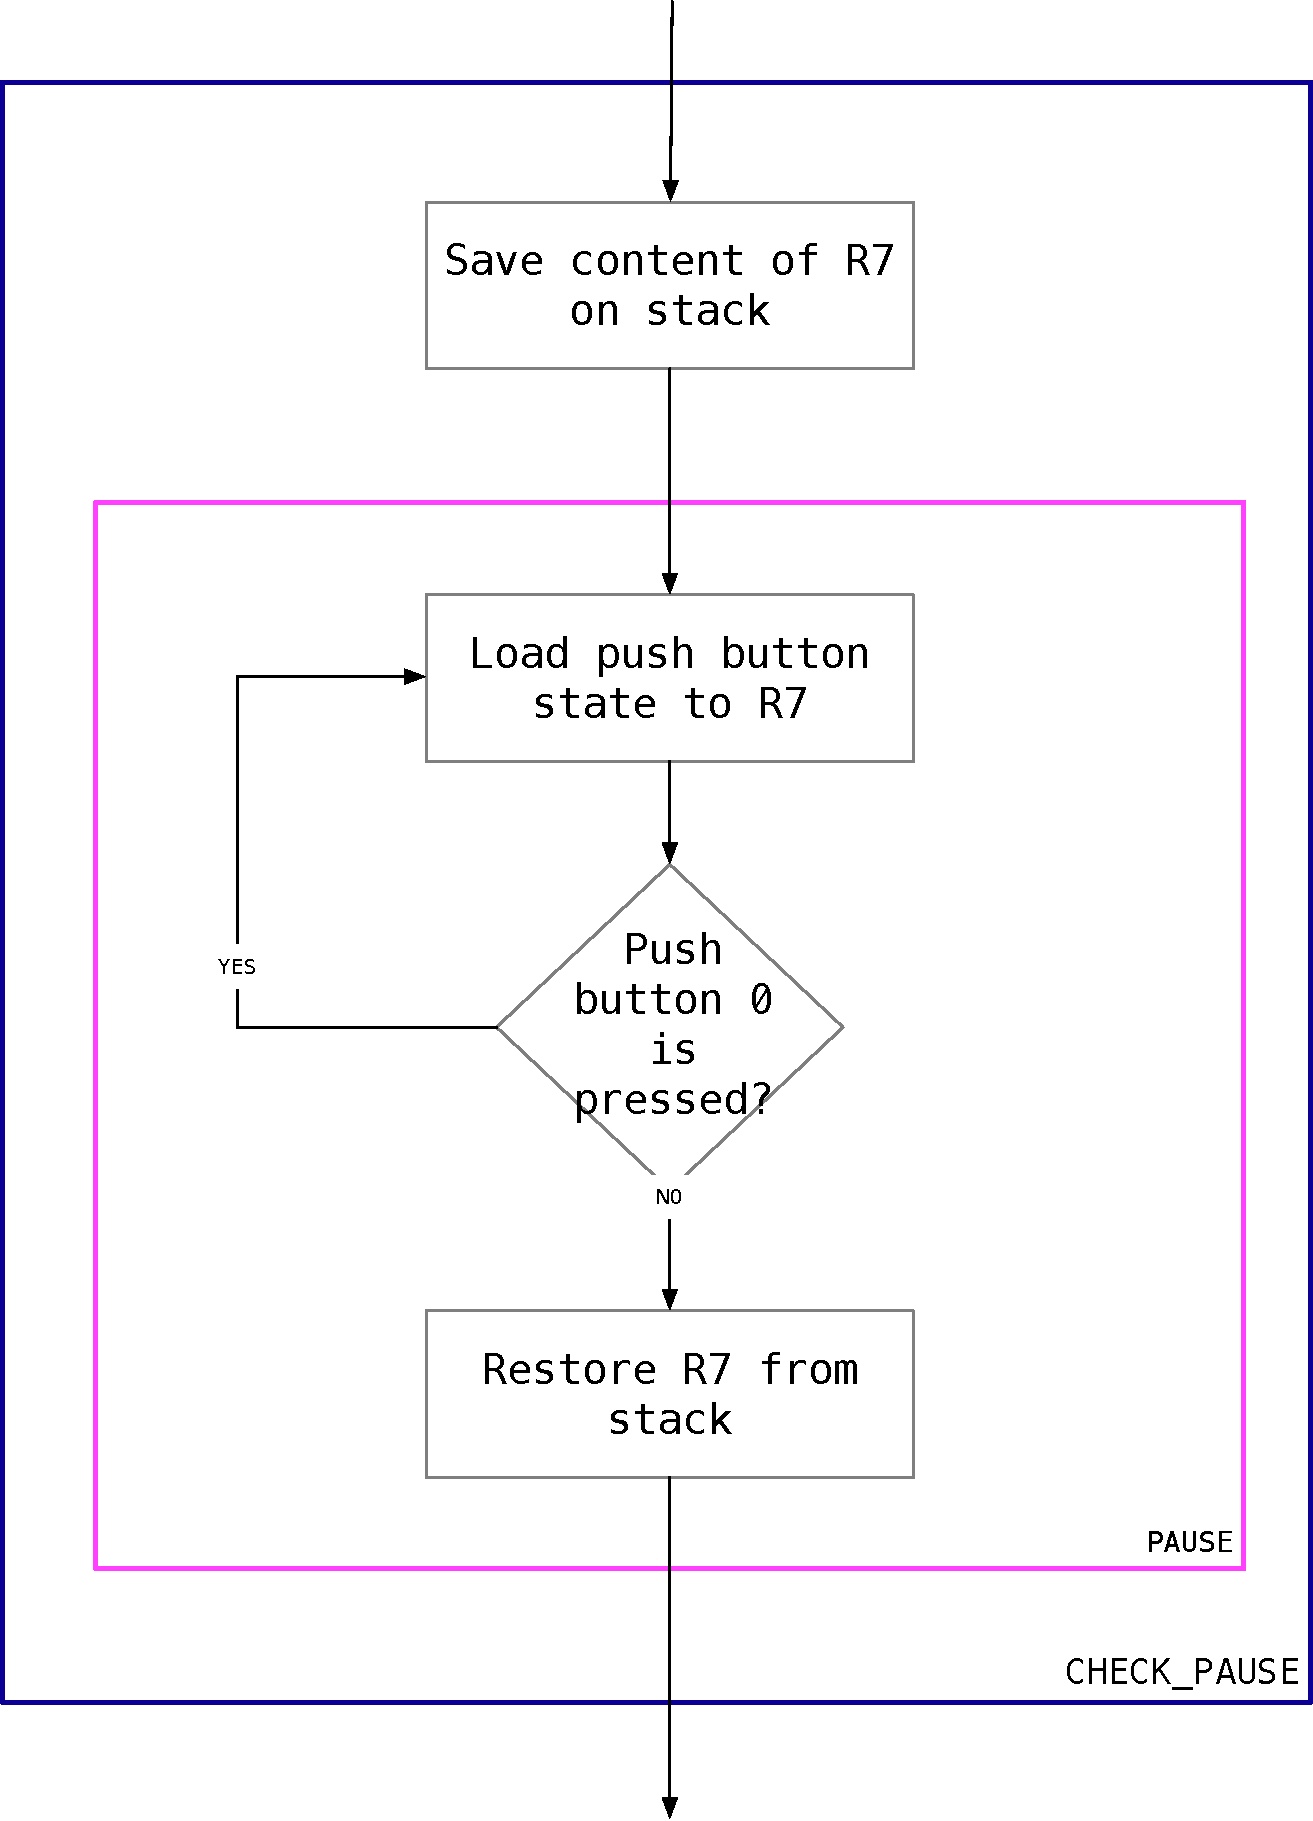
\includegraphics[scale=.45]{../images/check_pause.pdf}
		\caption{Flowchart of Check Pause Subroutine}
	\end{figure}
	\begin{figure}[h]
		\centering
		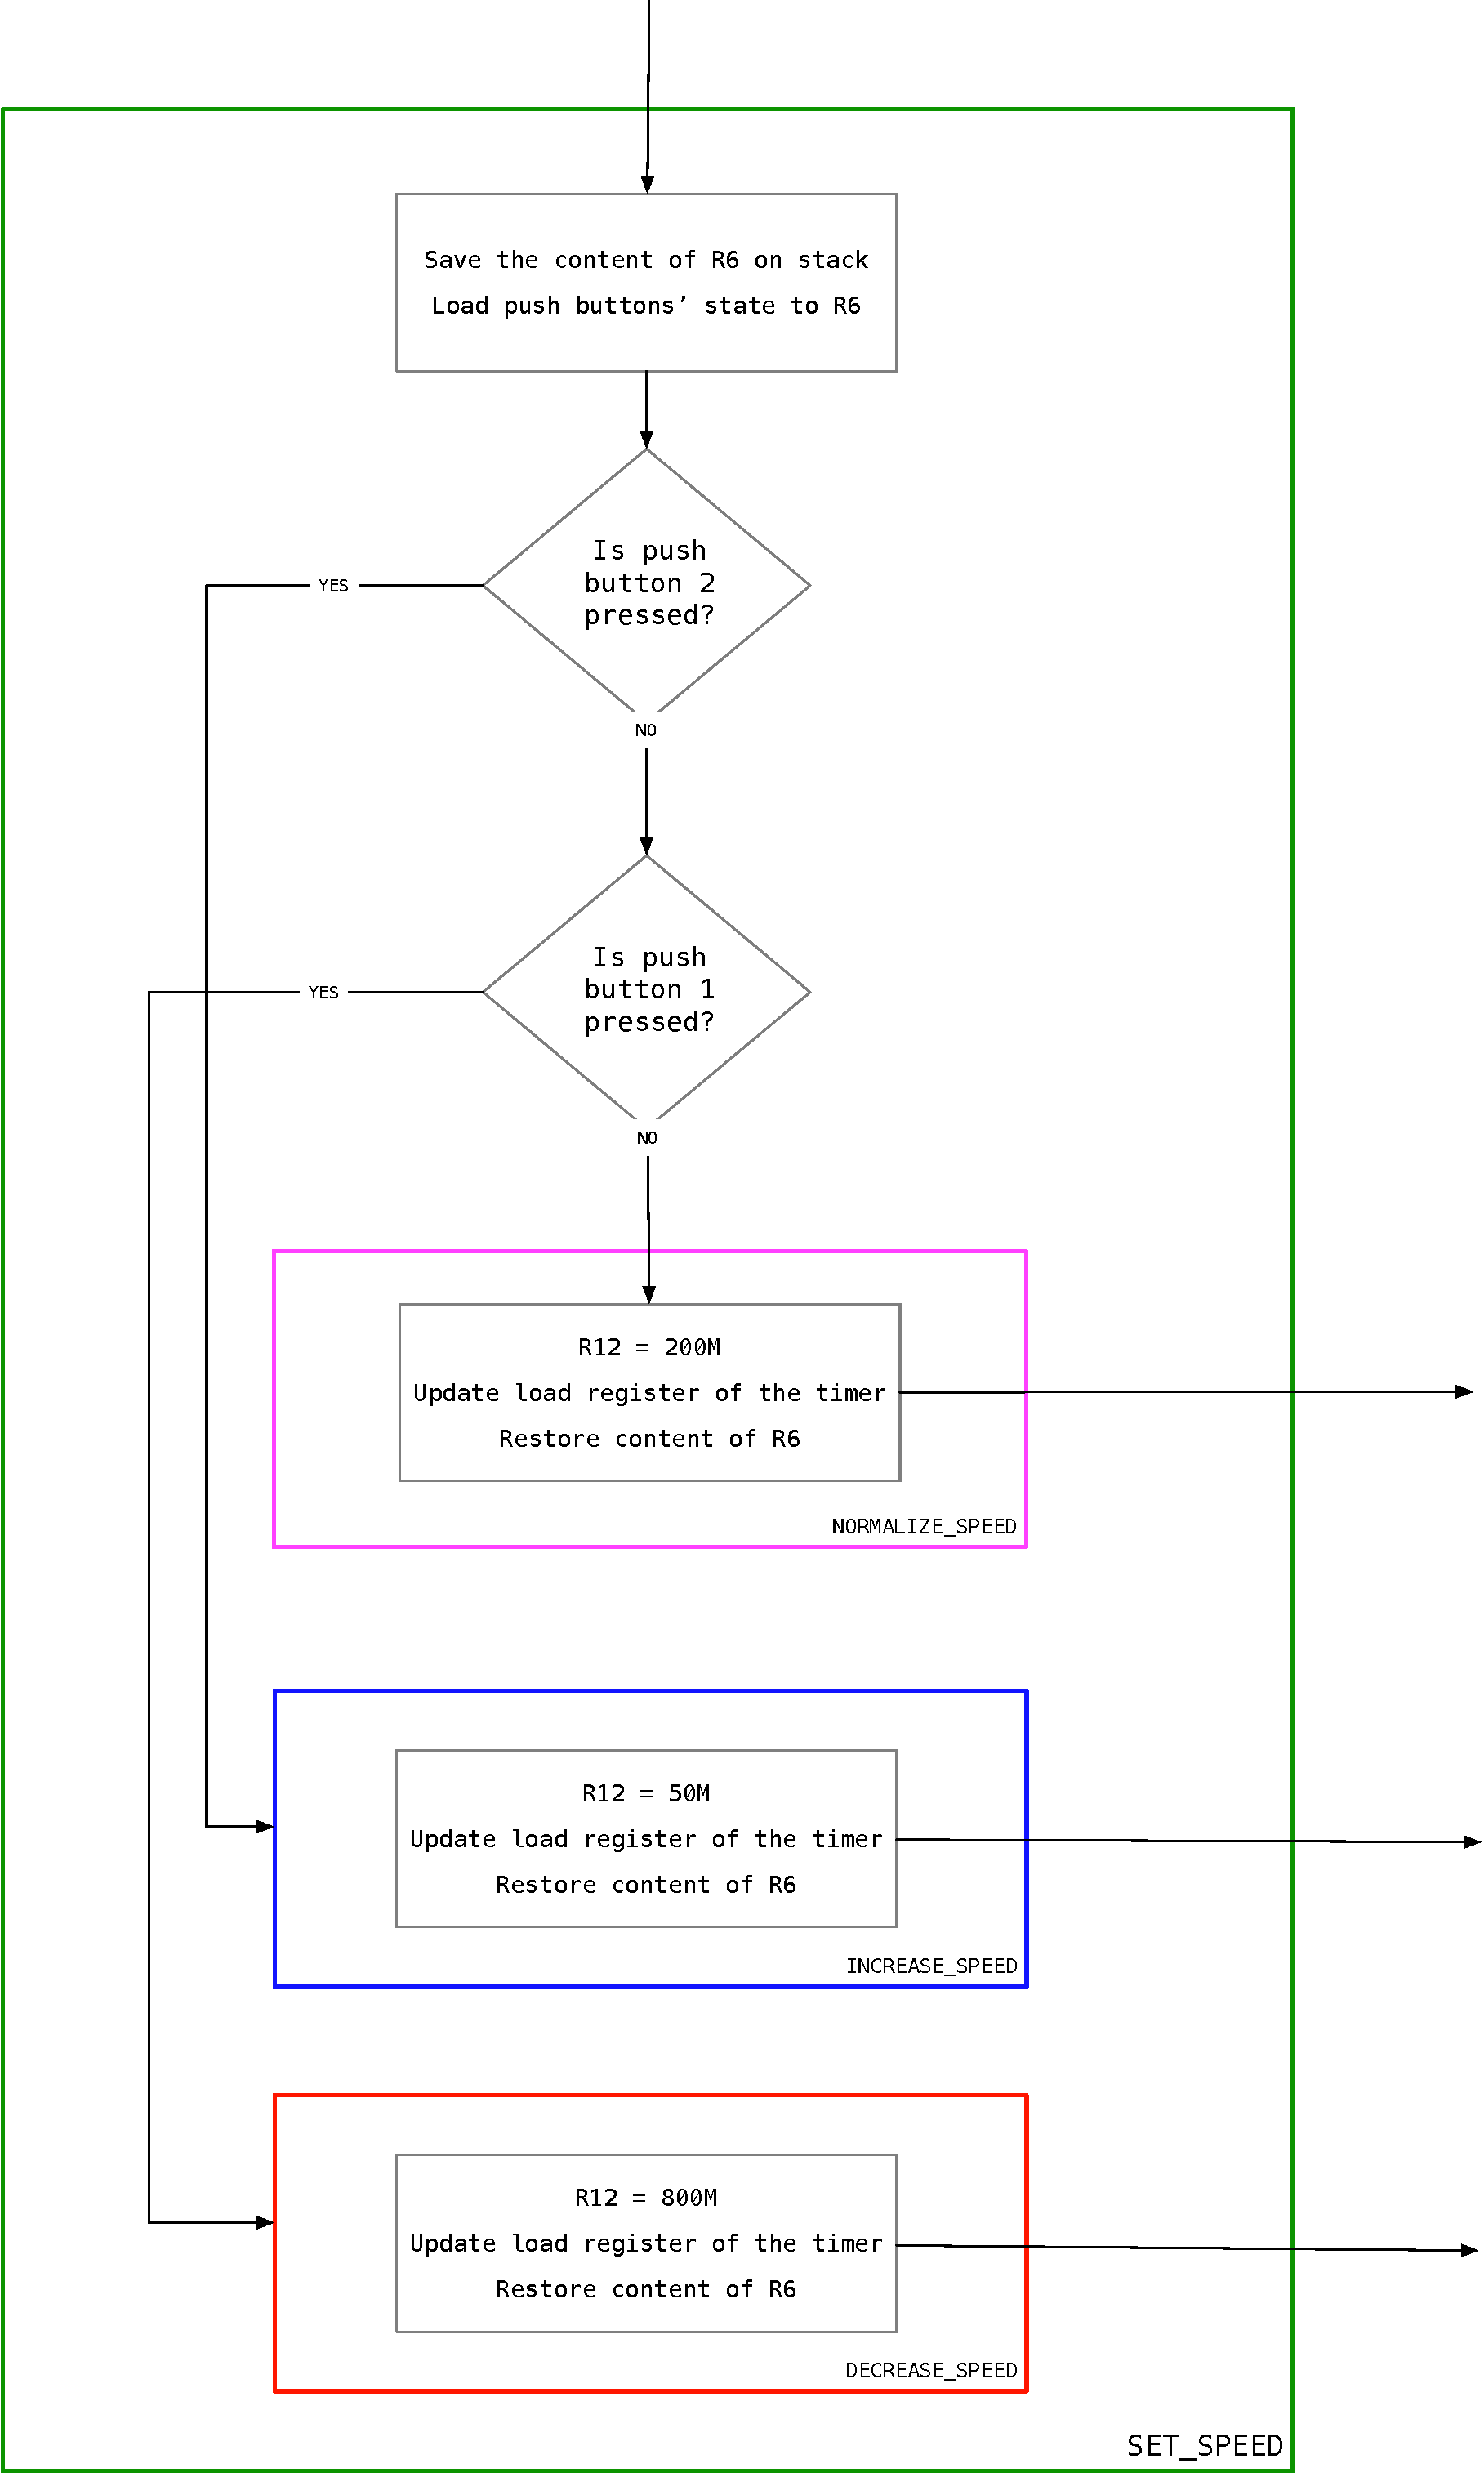
\includegraphics[scale=.35]{../images/set_speed.pdf}
		\caption{Flowchart of Set Speed Subroutine}
	\end{figure}
	\begin{figure}[h]
		\centering
		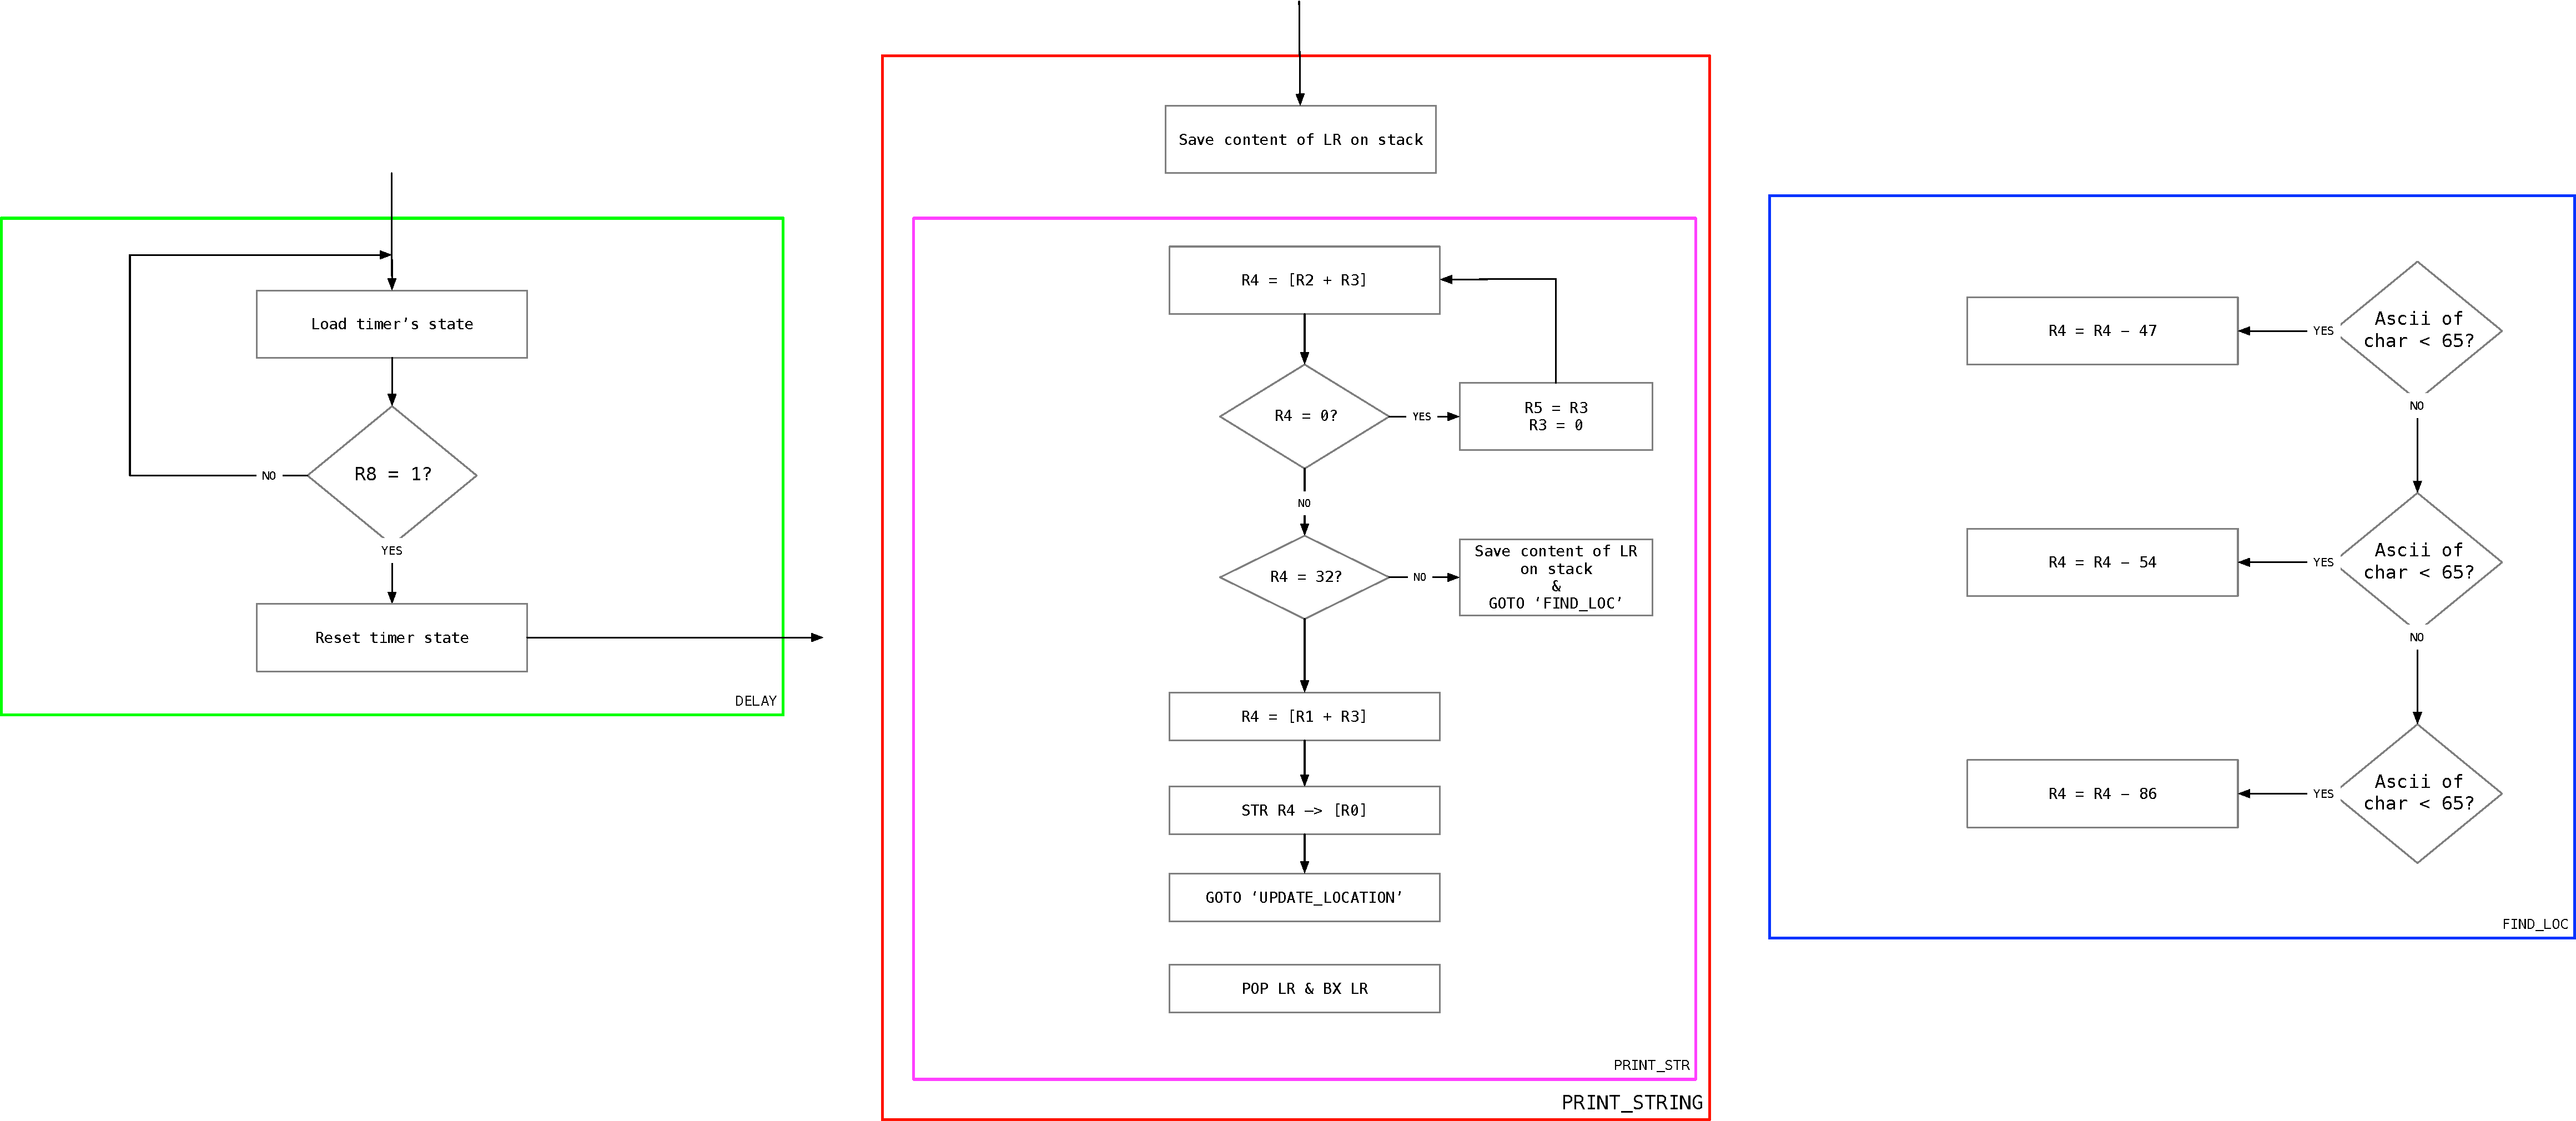
\includegraphics[scale=.15]{../images/print_string.pdf}
		\caption{Flowchart of Main Loop}
	\end{figure}


\end{document}